

%% LyX 2.2.1 created this file.  For more info, see http://www.lyx.org/.
%% Do not edit unless you really know what you are doing.
\documentclass[12pt, usenames, dvipsnames]{beamer}\usepackage[]{graphicx}\usepackage[]{color}
% maxwidth is the original width if it is less than linewidth
% otherwise use linewidth (to make sure the graphics do not exceed the margin)
\makeatletter
\def\maxwidth{ %
  \ifdim\Gin@nat@width>\linewidth
    \linewidth
  \else
    \Gin@nat@width
  \fi
}
\makeatother

\definecolor{fgcolor}{rgb}{0.345, 0.345, 0.345}
\newcommand{\hlnum}[1]{\textcolor[rgb]{0.686,0.059,0.569}{#1}}%
\newcommand{\hlstr}[1]{\textcolor[rgb]{0.192,0.494,0.8}{#1}}%
\newcommand{\hlcom}[1]{\textcolor[rgb]{0.678,0.584,0.686}{\textit{#1}}}%
\newcommand{\hlopt}[1]{\textcolor[rgb]{0,0,0}{#1}}%
\newcommand{\hlstd}[1]{\textcolor[rgb]{0.345,0.345,0.345}{#1}}%
\newcommand{\hlkwa}[1]{\textcolor[rgb]{0.161,0.373,0.58}{\textbf{#1}}}%
\newcommand{\hlkwb}[1]{\textcolor[rgb]{0.69,0.353,0.396}{#1}}%
\newcommand{\hlkwc}[1]{\textcolor[rgb]{0.333,0.667,0.333}{#1}}%
\newcommand{\hlkwd}[1]{\textcolor[rgb]{0.737,0.353,0.396}{\textbf{#1}}}%
\let\hlipl\hlkwb

\usepackage{framed}
\makeatletter
\newenvironment{kframe}{%
 \def\at@end@of@kframe{}%
 \ifinner\ifhmode%
  \def\at@end@of@kframe{\end{minipage}}%
  \begin{minipage}{\columnwidth}%
 \fi\fi%
 \def\FrameCommand##1{\hskip\@totalleftmargin \hskip-\fboxsep
 \colorbox{shadecolor}{##1}\hskip-\fboxsep
     % There is no \\@totalrightmargin, so:
     \hskip-\linewidth \hskip-\@totalleftmargin \hskip\columnwidth}%
 \MakeFramed {\advance\hsize-\width
   \@totalleftmargin\z@ \linewidth\hsize
   \@setminipage}}%
 {\par\unskip\endMakeFramed%
 \at@end@of@kframe}
\makeatother

\definecolor{shadecolor}{rgb}{.97, .97, .97}
\definecolor{messagecolor}{rgb}{0, 0, 0}
\definecolor{warningcolor}{rgb}{1, 0, 1}
\definecolor{errorcolor}{rgb}{1, 0, 0}
\newenvironment{knitrout}{}{} % an empty environment to be redefined in TeX

\usepackage{alltt}
\usepackage[T1]{fontenc}
\usepackage[utf8]{inputenc}
\setcounter{secnumdepth}{3}
\setcounter{tocdepth}{3}
\usepackage{url}
\ifx\hypersetup\undefined
\AtBeginDocument{%
\hypersetup{unicode=true,pdfusetitle,
bookmarks=true,bookmarksnumbered=false,bookmarksopen=false,
breaklinks=false,pdfborder={0 0 0},pdfborderstyle={},backref=false,colorlinks=false}
}
\else
\hypersetup{unicode=true,pdfusetitle,
bookmarks=true,bookmarksnumbered=false,bookmarksopen=false,
breaklinks=false,pdfborder={0 0 0},pdfborderstyle={},backref=false,colorlinks=false}
\fi
\usepackage{breakurl}
\usepackage{xspace}
\usepackage{array}
\usepackage{xcolor}

\newcommand{\ggplot}{\rf{ggplot()}\xspace}
\newcommand{\ggpp}{\rt{ggplot2}\xspace}
\newcommand{\sumi}{\sum_{i=1}^n}
\newcommand{\xbar}{{\overline{x}}}
\newcommand{\ybar}{{\overline{y}}}

\newcommand{\while}{{\tt while}\xspace}
\makeatletter

%%%%%%%%%%%%%%%%%%%%%%%%%%%%%% LyX specific LaTeX commands.
\providecommand{\LyX}{\texorpdfstring%
{L\kern-.1667em\lower.25em\hbox{Y}\kern-.125emX\@}
{LyX}}

%%%%%%%%%%%%%%%%%%%%%%%%%%%%%% Textclass specific LaTeX commands.
% this default might be overridden by plain title style
\newcommand\makebeamertitle{\frame{\maketitle}}%
% (ERT) argument for the TOC
\AtBeginDocument{%
\let\origtableofcontents=\tableofcontents
\def\tableofcontents{\@ifnextchar[{\origtableofcontents}{\gobbletableofcontents}}
\def\gobbletableofcontents#1{\origtableofcontents}
}

\renewenvironment{knitrout}{\setlength{\topsep}{0mm}}{} 

%%%%%%%%%%%%%%%%%%%%%%%%%%%%%% User specified LaTeX commands.
\usetheme{default}


%%%%%%%%%%%%%%%%%%%%%%%%%%%%%% User specified LaTeX commands.
% beamer slides are typicaly 12.8cm x 9.6 / 5.04 in x 3.8

\makeatother


\usepackage[utf8]{inputenc}
\usepackage[T1]{fontenc}
\usepackage[english]{babel}

%\usepackage{verbatim}

\usepackage[export]{adjustbox}

\usepackage{
    amsmath,
    amsfonts,
    etex,
    fancyvrb,
    graphicx,
    multicol,
    pifont,
    setspace,
    soul,
    spverbatim,
    textcomp,
    xcolor,
    xspace
}

\usepackage{tikz}
\usetikzlibrary{shadows}

%%%SETUP%%%
\hypersetup{
     colorlinks = true,
     linkcolor = blue,
     anchorcolor = blue,
     citecolor = blue,
     filecolor = blue,
     urlcolor = blue
     }
     
%%%THEOREMS%%%
\theoremstyle{example}
\newtheorem*{exercise}{Exercise}
\newtheorem*{question}{Question}
\newtheorem*{answer}{\emph{Answer}}
\newtheorem*{notation}{Notation}

%%%TWEAKS%%%
\setlength\arraycolsep{4pt}
\addtolength\fboxsep{10pt}
\setstretch{1.4}
\setbeamersize{description width=3em}
\setbeamersize{text margin left=.5cm,text margin right=.5cm} 
\renewcommand{\emph}{\alert}
\renewcommand{\arraystretch}{1.2}
\renewcommand{\tabcolsep}{4pt}
\setbeamercolor{alerted text}{fg=magenta}


\graphicspath{{img/}}

%for straight quotes in verbatim:
\usepackage{upquote,textcomp}

%turn off navigation symbols
\beamertemplatenavigationsymbolsempty
\setbeamertemplate{footline}[frame number]

%title page

\author
  [Dr.\ Irene Vrbik]
  {Dr.\ Irene Vrbik}

\date
  {}

\institute
  {University of British Columbia Okanagan \newline \texttt{irene.vrbik@ubc.ca}}
  
\definecolor{iyellow}{RGB}{255, 162, 23}
\definecolor{sgreen}{RGB}{118, 191, 138}

\newcommand{\yellow}[1]{\textcolor{iyellow}{#1}}
\newcommand{\red}[1]{\textcolor{red}{#1}}
\newcommand{\green}[1]{\textcolor{ForestGreen}{#1}}
\newcommand{\blue}[1]{{\textcolor{blue}{#1}}}
\newcommand{\orange}[1]{{\textcolor{orange}{#1}}}
\newcommand{\bblue}[1]{\textcolor{SteelBlue!90!gray}{#1}} % beamer blue
\newcommand{\purple}[1]{{\textcolor{purple}{#1}}}

\newcommand{\el}{\\[1em]\pause}
\newcommand{\nl}{\\[1em]}
\newcommand{\define}[1]{\textbf{\textcolor{orange}{#1}}}

%\newcommand{\answer}[1]{\textit{\textbf{\textcolor{iyellow}{#1}}}}

\newcommand{\command}[1]{\texttt{\textbf{\textcolor{DarkMagenta}{#1}}}}
\newcommand{\ipic}[2]{\includegraphics[width={#2}\textwidth]{#1}}
\newcommand{\cell}[1]{{\sf \textbf{\textcolor{DarkMagenta}{#1}}}}
\newcommand{\ra}{$\rightarrow$}

\newcommand{\ft}[1]{\frametitle{#1}}


\newenvironment{allintypewriter}{\ttfamily}{\par}
\newcommand{\bs}{$\backslash$}

\newcommand*\keystroke[1]{%
  \tikz[baseline=(key.base)]
    \node[%
      draw,
      fill=white,
      drop shadow={shadow xshift=0.25ex,shadow yshift=-0.25ex,fill=black,opacity=0.75},
      rectangle,
      rounded corners=2pt,
      inner sep=1pt,
      line width=0.5pt,
      font=\scriptsize\sffamily
    ](key) {#1\strut}
  ;
}

% timed answer
\newcommand{\tans}[2]{\textbf<#1>{\textit<#1>{{\color<#1>{iyellow}{#2}}}}}


\makeatletter
\g@addto@macro\normalsize{%
  \setlength\abovedisplayskip{0.4em}
  \setlength\belowdisplayskip{0.4em}
  \setlength\abovedisplayshortskip{0.2em}
  \setlength\belowdisplayshortskip{0.2em}
}
\makeatother


\newcommand{\cmark}{{\Large\color{green}\ding{51}}}%
\newcommand{\xmark}{{\Large\color{red}\ding{55}}}%

\newcommand{\pcmark}{\onslide<+->{\cmark}}
\newcommand{\pxmark}{\onslide<+->{\xmark}}

\newcommand{\by}{\overline{y}}
\newcommand{\ty}{\tilde{y}}

\newcounter{saveenumi}
\newcommand{\seti}{\setcounter{saveenumi}{\value{enumi}}}
\newcommand{\conti}{\setcounter{enumi}{\value{saveenumi}}}

\definecolor{dimgray}{rgb}{0.41, 0.41, 0.41}
\definecolor{blue(ncs)}{rgb}{0.0, 0.53, 0.74}
% R arguments/parameters
\newcommand{\rp}[1]{\textcolor{Green}{\tt #1}}
% R functions
\newcommand{\rf}[1]{\textcolor{BrickRed}{\tt #1}}
% R characters
\newcommand{\rc}[1]{\textcolor{blue(ncs)}{\tt #1}}
% R values and reserved words
\newcommand{\rv}[1]{\textcolor{RedViolet}{\tt #1}}
% R objects
\newcommand{\ro}[1]{\textcolor{dimgray}{\tt #1}} 
% R text/commans
\newcommand{\rt}[1]{\textcolor{dimgray}{\tt #1}}
\IfFileExists{upquote.sty}{\usepackage{upquote}}{}
\begin{document}


\renewenvironment{knitrout}{\setlength{\topsep}{0mm}}{}

\title[Data 301]{R Part IV - Statistics $t$-tests}

\makebeamertitle



\begin{frame}{Introduction}
\begin{itemize}
% \item Now that we covered the fundamental concepts of programing in R, we can discuss some  the important statistical analyses that are commonly performed with this software (and others).
 % \item Some of these methods we would have seen already in our Excel and Python unit, others will be seeing for the first time. 
 \item Today we will dive a little deeper into some of the statistical tools you may find yourself using in R.
 \vfill
\item While these tests are not specific to R, the specific syntax used throughout this lecture will be.
\vfill
\item As always, you can find the code used throughout this lecture on Canvas.
\vfill
\end{itemize}
\end{frame}

\begin{frame}[fragile]
\begin{itemize}
% http://www.sthda.com/english/wiki/comparing-means-in-r
% \item We begin with a basic statistical test for comparing continuous data.
% \vfill
\item More specifically we will be looking at the \rf{t.test()} function in R for the purpose of \alert{hypothesis testing}.
\vfill
\item We will focus on 
\begin{enumerate}
\item comparing one-sample mean to a  to a stipulated value,
\item comparing the means of two independent groups:
\item comparing the means of paired samples:
% \item \textcolor{gray}{comparing the means of more than two groups}
\end{enumerate}
\vfill
\end{itemize}
\end{frame}


\begin{frame}[fragile]{Hypothesis Testing}
Hypothesis testing is an essential procedure in statistics.
% \emph{Hypothesis testing} is used to determine if a relationship exists between two sets of data and make decisions/conclusions about that relationship.
\vfill
% \emph{Hypothesis testing is useful for}
Hypothesis tests are used in virtually every field of study, here are some applications to name just a couple:
\begin{enumerate}
\item in determining whether a value is below/above a certain threshold, eg. test if the average cadmium level in edible mushrooms is below the tolerable value of 3 mg/kg
\item in determining an effect in controlled experiments, eg. to compare a new medical treatment to a placebo. %eg. to determine whether  monthly energy cost for families has changed from the previous year}
\item in determining effectiveness of marketing, eg. is this years sales better than the previous year? %identifying customer buying properties, online advertising optimization.
% \item eg.
% do less than half the adults in a certain area favour the construction of an outdoor rink? %in determining %if data sets match a model, understanding scientific process based on collected data values, analysis of study data.
\end{enumerate}
\vfill
\end{frame}



\begin{frame}[fragile]{Background}
\emph{Hypothesis testing} is form of inferential statistics.
\begin{itemize}
\item \define{Statistical inference} involves forming judgements on a population of interest based on a random sample drawn from that population.
\item In contrast to descriptive statitistcs---which  does not allow us to make conclusions beyond the data we have observed--- inferential statitics aims at using information provided by the sample to infer and make predictions about a population from which it came. 
% \item This form of statistics can be contrasted with descriptive statistics. Descriptive statistics is solely concerned with properties of the observed data, and it does not rest on the assumption that the data come from a larger population.
\end{itemize}
\end{frame}

\begin{frame}[fragile]{Background}
\begin{itemize}
\item The general family of $t$-tests refer to statistical hypothesis tests which rely on the bell-shaped $t$-distribution.  
\vfill
\item While the complete collection of $t$-tests along with their mathematical justification are beyond the score of this course, %we will discuss the common  problem %s than the ones discussed today
%or the purpose of this lecture, 
we highlight a commonly used  $t$-test for performing inference on population \textit{means}.
\vfill
%, we will focus 
% \item Popular tests include:
% \begin{itemize}
% \item Determining if a relationship exists between two sets of data and make decisions/conclusions about that relationship.
% \item 
% \end{itemize}
\end{itemize}
% \vfill
% \emph{Hypothesis testing is useful for}
% \begin{enumerate}
% \item \emph{business} in determining effectiveness of marketing, identifying customer buying properties, online advertising optimization.
% \item \emph{science and social science} in determining if data sets match a model, understanding scientific process based on collected data values, analysis of study data.
% \end{enumerate}
% \vfill
\end{frame}
%%%%%%%%%%%%%%%%%%%%%%%%%%%%%%%%%%%%%%%%%%%%%%%%%%%%%%%%




\begin{frame}[fragile]{One-sample $t$-test}{Assumptions}
There are assumptions that need to be met before performing $t$-test.
% For the one sample:
\begin{enumerate}
\item Population of interest is normally distributed.
\item Independent random samples are taken.
\end{enumerate}
\vfill
% For the two sample case:
% \begin{enumerate}
% \item The two samples are independent.
% \item Populations of interest are normally distributed.
% \end{enumerate}
While there are statistical methods for %to empirically
testing assumptions (eg. Shapiro-Wilk test for normality), %see the above Normality tests section.
for breverity, we assume that they have been met. 
\vfill
\end{frame}
%%%%%%%%%%%%%%%%%%%%%%%%%%%%%%%%%%%%%%

\begin{frame}[label=normal]{Normal distribution}
\begin{itemize}
\item The normal distribuiton is the most  widely used  perhaps the most well recognizable distribution by it's  ``bell-shape". 
\vfill
\item The normal distribution is characterized by two parameters: its mean ($\mu$) and standard deviation ($\sigma$).
\begin{itemize}
\item the \define{mean} provides the location of the bell's center
\item and the \define{standard deviation} describes how spread out, or `fat', that bell shape is. 
\end{itemize}
\end{itemize}
\vfill
\end{frame}



\begin{frame}[fragile]{The Normal Distribution}
\begin{knitrout}\footnotesize
\definecolor{shadecolor}{rgb}{0.969, 0.969, 0.969}\color{fgcolor}

{\centering 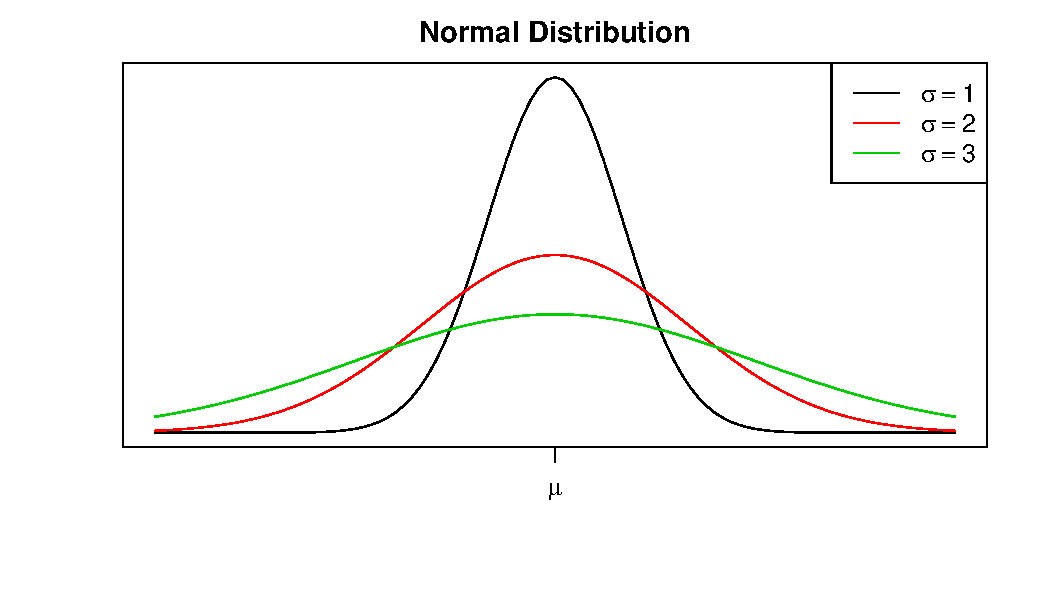
\includegraphics[width=\maxwidth]{figure/beamer-unnamed-chunk-1-1} 

}



\end{knitrout}
The tails of this distribution actually run from -$\infty$ to $\infty$.
\end{frame}

\begin{frame}[fragile]{Null Hypothesis}
\begin{itemize}
\item For the one sample problem, we may wish to test the hypothesis that the population is centered at some supposed value $\mu_0$.
\vfill
\item In more statistical terms, we may wish to test the \define{null hypothesis} of  $H_0: \mu = \mu_0$.
\vfill
\item In this course the null hypothesis, $H_0$, always contains a statement of no change ($=$). *This is not universal across textbooks. \nl
\end{itemize}
\end{frame}

\begin{frame}[fragile]{Alternative Hypothesis}
\begin{itemize}
\item $H_0$ is tested against a competing statement called the \define{alternative hypothesis} $H_1$ (sometimes written $H_A$).
\item We can either make this alternative one or two-sided:
\begin{itemize}
\item[] $H_1: \mu \neq \mu_0$ (two-sided)
\item[] $H_1: \mu < \mu_0$ (one-sided, lower-tailed)
\item[] $H_1: \mu > \mu_0$ (one-sided, upper-tailed)
\end{itemize}
\item $H_0$ and $H_1$ should always be written in terms of the \textit{population} parameters (in this case $\mu$).
\end{itemize}
\end{frame}



\frame{
\frametitle{Alternative Hypothesis} 

\begin{itemize}
\item  The direction of our alternative hypothesis will depend on the situation at hand.
\vfill
 \item A two-sided alternative may be preferred if %you no suspicion of specific direction (i.e. $>$ or $<$ than) in advanced.\nl
 a deviation in either direction is just as grave.
\begin{itemize}
\item  eg. to compare a new medical treatment to a placebo (we care both if the treatment is effective and if it is harmful). %eg. to determine whether  monthly energy cost for families has changed from the previous year}
% \item For example, if we are trying to determine the right dose for a drug, we want to make sure we dont overmedicate (which could lead to adverse health affects) or undermedicate (which would render our drug ineffective).
\end{itemize}
\vfill
\end{itemize}
}



\frame{
\frametitle{Alternative Hypothesis} 

\begin{itemize}

 \item One-sided alternatives may be preferred if %you no suspicion of specific direction (i.e. $>$ or $<$ than) in advanced.\nl
 results of your test are only relavent in one direction.
\begin{itemize}
\item eg. is this years sales better than the previous year? (if yes, employees get a bonus, if not, nothing happens) %identifying customer buying properties, online advertising optimization.
\item eg. do less than half the adults in a certain area favour the construction of an outdoor rink? %in determining %if data sets match a model, understanding scientific process based on collected data values, analysis of study data.
\end{itemize}
\end{itemize}
}


\begin{frame}[fragile]{One Sample Test Example}
\begin{itemize}
% \item A \emph{one sample test} can be used to compare a sample to a model or known population/estimate.
% \vfill
\item This test can be used to determine if the sample mean $\xbar$ is \textit{significantly} different then some hypothesized value $\mu_0$.
\vfill
\item Note that with any sample, it would be rare that a sample mean be \textit{exactly} equal to the hypothesized value.
\begin{itemize}
\item eg. even if the average height of men on campus is 69.3 in, a sample of 50 students may yeild a sample mean of 68.9 in.
\end{itemize}
% \item As an example, let's test if the average mileage {\tt cars} is different than 10.5km/L.
\vfill
\item The question therefore becomes: how far does my sample mean need to stray from the hypothesized value before I begin to question it's validity?
\end{itemize}
\end{frame}
%%%%%%%%%%%%%%%%%%%%%%%%%%%%%%%%%%%%%%%%%%%%%%%%%%%%%%%%%%%%%%%%%%%%%%%%%%%%%%%%%%%%%%%%%%%%%%%%%%%%
% 
% 
% \begin{frame}[fragile]{One Sample Test Example}
% \vfill
% \begin{itemize}
% \item Consider the scenario where this collection of cars \textit{is} in fact sampled from a population having a mean average mileage equal to 10.5km/L. (i.e. our null hypothesis is correct).
% \item Based on the randomness of sampling, it would be unrealistic to expect that our sample would produce an $\xbar$ exactly equal to 10.5km/L.\nl
% \item Therefore we should expect some plausible wiggle room around our hypothesized value of 10.5 which we would deem close enough.\nl
% \end{itemize}
% \end{frame}
% 
% 
% \begin{frame}[fragile]{One Sample Test Example}
% \vfill
% \begin{itemize}
% \item On the contrary, once we pass a certain threshold, we could determine that our sample is inconsistent with our hypothesis. 
% \item That threshold should of course depend on the problem at hand.
% \item For example, we would explect the threshold for the black curve on \hyperlink{normal}{this} slide should would be more strict than the thresold for the green curve. 
% \end{itemize}
% \end{frame}






%%%%%%%%%%%%%%%%%%%%%%%%%%%%%%%%%%%%%%%%%%%%%%%%%%%%%%%%%%%%%%%%%%%%%%%%%%%%%%%%%%%%%%%%%%%%%%%%%%%%
\begin{frame}[fragile]{One Sample Test: Calculate Test Statistic}
To answer this question we use a \define{test statistic} which follows some known distribution.
\vfill
For the one sample test the $t$-test statistic is calculated as:
\begin{equation}\label{teststat}
t = \dfrac{\xbar - \mu_0}{\dfrac{s}{\sqrt n}}
\end{equation}
\vfill
where $\xbar$ is the sample mean, $s$ is the sample standard deviation, $n$ is the sample size, and $\mu_0$ is the hypothesized mean value.
\vfill
As alluded to earlier, this statistic follows a $t$-distribution.
\end{frame}


\begin{frame}[fragile]
The distribution of \eqref{teststat} looks like this:
\begin{knitrout}\footnotesize
\definecolor{shadecolor}{rgb}{0.969, 0.969, 0.969}\color{fgcolor}

{\centering 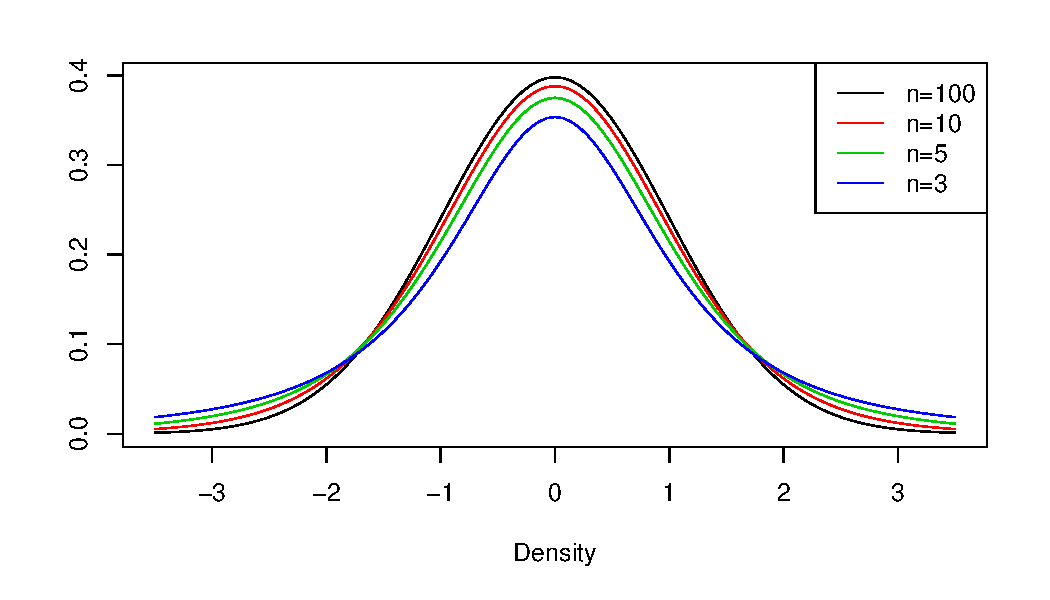
\includegraphics[width=\maxwidth]{figure/beamer-unnamed-chunk-2-1} 

}



\end{knitrout}
It's shape is determined by the degrees of freedom parameter $\nu = n- 1$ (the smaller $n$ is, the fatter/more squished it appears)
\end{frame}


\begin{frame}[fragile]{One Sample Test Example}
\begin{itemize}
\item Consider the {\tt car\_data.csv} file uploaded to Canvas.
\begin{knitrout}\footnotesize
\definecolor{shadecolor}{rgb}{0.969, 0.969, 0.969}\color{fgcolor}\begin{kframe}
\begin{alltt}
\hlstd{car_data} \hlkwb{<-} \hlkwd{read.csv}\hlstd{(}\hlstr{"data/car_data.csv"}\hlstd{)}
\end{alltt}
\end{kframe}
\end{knitrout}


\vfill
\item This data contains information on 8 variables from 30 cars.
\vfill
\item We would like to test if the average mileage ({\tt km.L}) differs from 10km/L.
\vfill\end{itemize}
\end{frame}

%%%%%%%%%%%%%%%%%%%%%%%%%%%%%%%%%%%%%%%%%%%%%%%%%%%%%%%%%%%%%%%%%%%%%%%%%%%%%%%%%%%%%%%%%%%%%%%%%%%%
\begin{frame}[fragile]{Step 1: Hypotheses Statements}
\begin{itemize}
% \item  Alternatively hypothesis ($H_A$) can be one sided ($<$ or $>$) or two sided ($\neq$).
% \begin{align*}
% H_0: \mu = \mu_0& \quad vs  &H_A: \mu > \mu_0
% \end{align*}
% \vfill
\item The first step is always to write the null and alternative hypothesis:
\begin{align*}
H_0: \mu = 10& \quad vs  &H_1: \mu \neq 10
\end{align*}
(i.e. our hypothesized value is $\mu_0 = 10$).
\item Analogous to a courtroom, we believe $H_0$ is true until evidence (in the form of data) suggests otherwise.
% \item To determine our threshold which determines how far our sample mean needs to depart from 10.5 before we no longer believe $H_0$ is true, we need a \define{test statistic}.  
%More generically, we use $H_0: \mu = \mu_0$ where $\mu_0$ is the hypothesized mean.
\vfill
\end{itemize}
\end{frame}
%%%%%%%%%%%%%%%%%%%%%%%%%%%%%%%%%%%%%%%%%%%%%%%%%%%%%%%%%%%%%%%%%%%%%%%%%%%%%%%%%%%%%%%%%%%%%%%%%%%%


\begin{frame}[fragile]{Step 2: calculate test statitic}\label{cartobs}
\begin{itemize}
\item Step 2 is to calculate our test statistic:
\begin{align*}
t = \dfrac{\xbar - \mu_0}{\dfrac{s}{\sqrt n}}
\end{align*}
N.B. once we plug in values to our test statistic, we call it the \textit{observed} test statistic $t_{obs}$
% \begin{align*}
% t_{obs} = \dfrac{mean(car_data$km.L) - mu0}{\dfrac{sd(car_data$km.L))}{\sqrt nrow(car_data)}}
% \end{align*}


\begin{align*}
t_{obs} = \dfrac{10.3553333 - 10}{\dfrac{1.210354}{\sqrt 30}} = 1.6079931
\end{align*}
\end{itemize}
\end{frame}


\begin{frame}[fragile]{Step 2: calculate test statitic}
\begin{knitrout}\footnotesize
\definecolor{shadecolor}{rgb}{0.969, 0.969, 0.969}\color{fgcolor}\begin{kframe}
\begin{alltt}
\hlstd{mu0} \hlkwb{=} \hlnum{10} \hlcom{# hypothesize value}
\hlstd{n} \hlkwb{=} \hlkwd{nrow}\hlstd{(car_data)}
\hlstd{tobs} \hlkwb{=} \hlstd{(}\hlkwd{mean}\hlstd{(car_data}\hlopt{$}\hlstd{km.L)}\hlopt{-} \hlstd{mu0)}\hlopt{/}\hlstd{(}\hlkwd{sd}\hlstd{(car_data}\hlopt{$}\hlstd{km.L)}\hlopt{/}\hlkwd{sqrt}\hlstd{(n))}
\hlstd{tobs}
\end{alltt}
\begin{verbatim}
## [1] 1.607993
\end{verbatim}
\end{kframe}
\end{knitrout}
\end{frame}


\begin{frame}[fragile]{Step 3: convert to a $p$-value}
\begin{itemize}
\item Step 3 is to convert this test statistic to a $p$-value.
\item A $p$-value is calculated as:
\begin{itemize}
\item[] $2*P(t > \mid t_{obs}\mid)$ if $H_1: \mu \neq \mu_0$ (two-sided)
\item[] $P(t < t_{obs})$ if $H_1: \mu < \mu_0$ (one-sided, lower-tailed)
\item[] $P(t > t_{obs})$ if $H_1: \mu > \mu_0$ (one-sided, upper-tailed)
\end{itemize}
Where
\begin{align*}
t = \dfrac{\xbar - \mu_0}{\dfrac{s}{\sqrt n}} 
\end{align*}
is a $t$-distributed random variable with $n-1$ degrees of freedom.
\end{itemize}
\end{frame}




\begin{frame}[fragile]{Step 3: convert to a $p$-value}\label{carpval}
We can visualize this probability as the following area underneath the curve:
\begin{knitrout}\footnotesize
\definecolor{shadecolor}{rgb}{0.969, 0.969, 0.969}\color{fgcolor}

{\centering 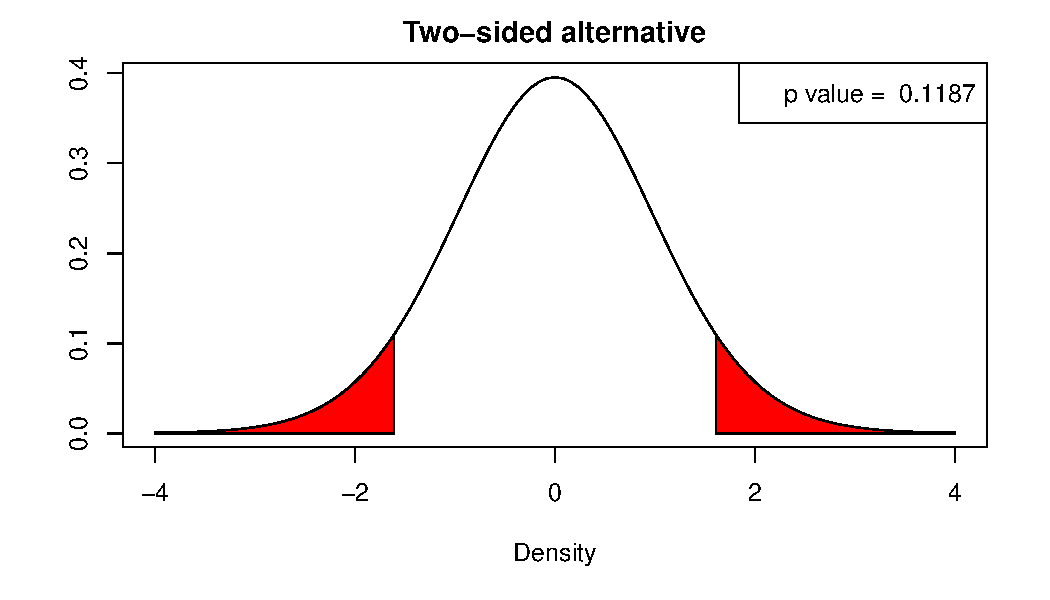
\includegraphics[width=\maxwidth]{figure/beamer-unnamed-chunk-5-1} 

}



\end{knitrout}
\end{frame}



\begin{frame}[fragile]{Step 3: convert to a $p$-value}\label{lpval}
Had we stated the  one-sided lower tailed alternative, our p-value would have been
\begin{knitrout}\footnotesize
\definecolor{shadecolor}{rgb}{0.969, 0.969, 0.969}\color{fgcolor}

{\centering 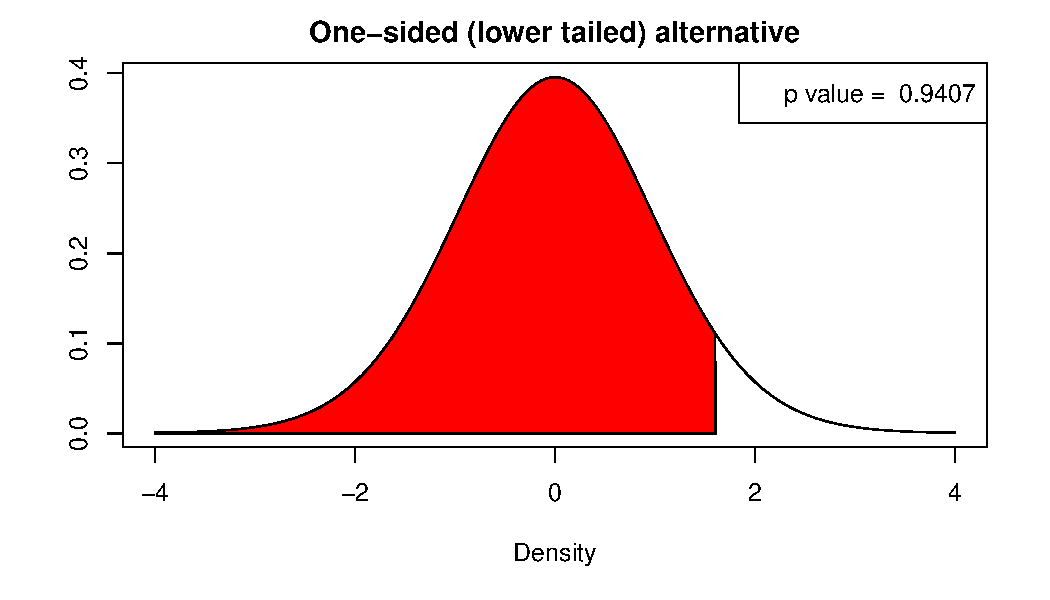
\includegraphics[width=\maxwidth]{figure/beamer-unnamed-chunk-6-1} 

}



\end{knitrout}
\end{frame}




\begin{frame}[fragile]{Step 3: convert to a $p$-value}\label{upval}
Had we stated the  one-sided upper tailed alternative, our p-value would have been
\begin{knitrout}\footnotesize
\definecolor{shadecolor}{rgb}{0.969, 0.969, 0.969}\color{fgcolor}

{\centering 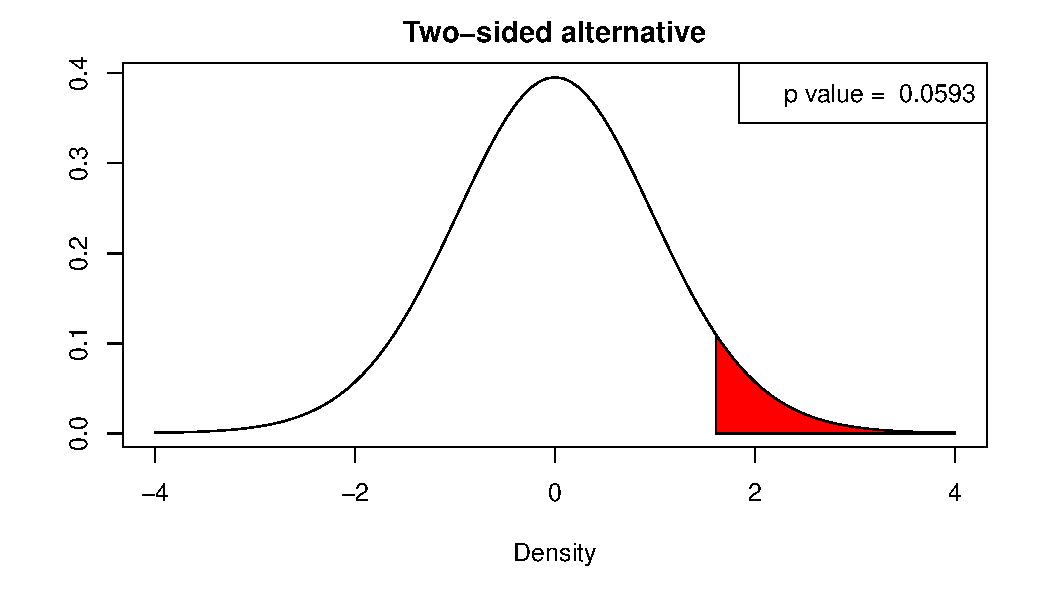
\includegraphics[width=\maxwidth]{figure/beamer-unnamed-chunk-7-1} 

}



\end{knitrout}
\end{frame}


 \begin{frame}[fragile]{Step 4: State Conclusion}
 \begin{itemize}
 \item Based on the evidence (ie data presented by the sample) we must decide whether or not we {reject} the hyptohesis or not. 
 \vfill
 \item This decision depends on our \define{confidence level},  often expressed as 1-$\alpha$, with $\alpha$ begin the \define{significance level}.
 \vfill
 \item The standard confidence level is 0.95 (ie. $\alpha = 0.05$)\footnote[frame]{unless stated otherwise, you may always assume $\alpha =0.05$}
$$
\text{Conclusion }=
\begin{cases}
\text{\emph{reject }}  H_0 & \text{if } \text{$p$-value } \leq \alpha\\
\text{\emph{fail to reject }}  H_0 & \text{if } \text{$p$-value } > \alpha
\end{cases}
$$
 \end{itemize}
\end{frame}


 \begin{frame}[fragile]{A note on stating conclusion}
 \begin{itemize}
 % \item Notice the language of our conclusions. Namely, we either reject or \textit{fail to reject} the null hypothesis $H_0$
 % \vfill
 \item Unless we have a complete sensus of the entire population we can \emph{never} say that a given null hypothesis is true.
 \vfill
 \item Our conclusion for our car example may be written:
 \begin{quote}
 Since the $p$-value (=0.1187) is greater than the significance level ($\alpha = 0.05$), 
 we \underline{fail to reject $H_0$}.  Therefore, there is  insufficient evidence to suggest that the average car mileage differs from 10.
 % we \underline{reject the null hypothesis}.  Therefore there is significant evidence to suggest that the average car mileage differs from mu0.
 \end{quote}
 \item Notice how we add context to this decision by referencing the alternative hypothesis in the context of the original problem.
 \end{itemize}
\end{frame}

%%%%%%%%%%%%%%%%%%%%%%%%%%%%%%%%%%%%%%%%%%%%%%%%%%%%%%%%%%%%%%%%%%%%%%%%%%%%%%%%%%%%%%%%
\begin{frame}[fragile]{Decision and Conclusion (using $P$-value)}
More generically, 
\vfill
If \alert{$p$-value $> \alpha$}, our decision/conclusion would be:
\begin{enumerate}
\item \alert{Fail to reject the null hypothesis}.
\item There is insufficient  evidence to suggest that the mean value is less than/greater than/different than the test value (will depend on alternative hypothesis)
\end{enumerate}
\end{frame}

\begin{frame}[fragile]{Decision and Conclusion (using $P$-value)}
\vfill

If \alert{$p{\rm-value} \leq \alpha$}, %the probability of seeing a sample mean more exteme than $\xbar$ is unlikely.
our decision/conclusion would be:
\begin{enumerate}
\item \alert{Reject the null hypothesis}.
\item There is statistically significant evidence to suggest that the mean value is less than that/greater than/ different than the test value  (will depend on alternative hypothesis).
\end{enumerate}
\vfill
\end{frame}
%%%%%%%%%%%%%%%%%%%%%%%%%%%%%%%%%%%%%%%%%%%%%%%%%%%%%%%%%%%%%%%%%%%%%%%%%%%%%%%%%%%%%%%%%



 \begin{frame}[fragile]{A note on the confidence levels}
 \begin{itemize}
 \item Loosely speaking we can view $\alpha$ as our adopted risk when performing this test.
 \vfill
 \item That is to say, if the null hypothesis is true, 5\% of the test we conduct under these conditions will result in the conclusion to reject the null hypothesis.
 \vfill
 \item We refer to this type of mistakes as Type 1 errors.
 \vfill
 \end{itemize}
\end{frame}



% \begin{frame}[fragile]
% \begin{itemize}
% \item If the hypothesis is true, there is only a 5\% chance that our test statistic falls in the area in red.  
% \item This may seem like a reasonable way to determine our threshold for believing $H_0: \mu = mu0$. 
% <<echo=FALSE>>=
% this <- t.test(x=car_data$km.L,
%         alternative=c("two.sided"), mu=mu0)
% high = this$statistic*sd(car_data$km.L)/sqrt(n) + mu0
% low = this$statistic*sd(car_data$km.L)/sqrt(n) - mu0
% @
%  \item To put numbers to this example, if $\xbar$ is less than low or bigger than high we will no longer believe the null hypothesis that the average gas mileage for this population of cars is equal to 10km/L. 
% \end{itemize}
% \end{frame}
% 
% \begin{frame}[fragile]
% \begin{itemize}
% \item Indeed this line of thinking is exactly what we follow when forming conclusions for a \textit{two-sided} \rf{t.test}. 
% \item  A similar argument can be made for one-sided tests:
% \vfill
% <<echo=FALSE, fig.height=3>>=
% par(mfrow=c(1,2))
% 
% xmin <- -3.5
% ntobs <- qt(0.025, df=29)
% ptobs <- qt(0.975, df=29)
% car_data <- read.csv("data/car_data.csv")
% n <- nrow(car_data)
% cord.x <- c(xmin,seq(xmin,ntobs,0.01),ntobs)
% cord.y <- c(0,dt(seq(xmin,ntobs,0.01), df=n-1),0)
% 
% # Make a curve
% curve(dt(x,df=n-1), xlim=c(xmin,abs(xmin)), xlab='Density',
%       main="Lower-tailed alternative", ylab="")
% 
% # Add the shaded area.
% polygon(cord.x,cord.y,col=2)
% #legend("topright", fill="skyblue", legend = "p-value")
% 
% 
% # Make a curve
% curve(dt(x,df=n-1), xlim=c(xmin,abs(xmin)), xlab='Density',
%       main="Upper-tailed alternative", ylab="")
% 
% 
% # Create data for the area to shade in the upper tail
% cord.x <- c(ptobs,seq(ptobs, abs(xmin),0.01),abs(xmin))
% cord.y <- c(0,dt(seq(ptobs,abs(xmin),0.01), df=n-1),0)
% polygon(cord.x,cord.y,col=2)
% @
% \item This area in red is sometimes referred to as the \define{rejection region}.
% \end{itemize}
% \end{frame}

\begin{frame}{Hypothesis testing in R}
\begin{itemize}
\item Now that we have a basic understanding of what these tests are doing, lets  code them up in R.  The general syntax:
\begin{center}
\rt{\rf{t.test}(\rp{x}=mydata,\rp{alternative}="two.sided",\rp{mu} =} $\mu_0$ \rt{,\rp{conf.level}=0.95,...)}
\end{center}
\item The default \rp{alterative} is \ro{"two.sided"} with the options \ro{"less"}, or \ro{"greater"}.
\item The default \rp{conf.level} = 0.95 (usually what we want)
\item To see the help file on this function, we type \rt{?t.test}.

\end{itemize}
\end{frame}




\begin{frame}[fragile]{One Sample Test: Cars Example}
The following code will  perform a one-sample $t$-test which tests:
\begin{align*}
H_0: \mu = 10& \quad \quad vs  &H_1: \mu \neq 10
\end{align*}
\begin{knitrout}\footnotesize
\definecolor{shadecolor}{rgb}{0.969, 0.969, 0.969}\color{fgcolor}\begin{kframe}
\begin{alltt}
\hlstd{car_data} \hlkwb{<-} \hlkwd{read.csv}\hlstd{(}\hlstr{"data/car_data.csv"}\hlstd{)}\hlcom{# read in the data}
\hlstd{mu0} \hlkwb{=} \hlnum{10} \hlcom{# hypothesize value}
\hlkwd{t.test}\hlstd{(}\hlkwc{x}\hlstd{=car_data}\hlopt{$}\hlstd{km.L,}             \hlcom{# sample mileage}
       \hlkwc{alternative}\hlstd{=}\hlstr{"two.sided"}\hlstd{,}  \hlcom{# two-side H_A}
       \hlkwc{mu}\hlstd{=mu0)} \hlcom{# set the hypothesized value mu0 }
\hlcom{# since a two-sided test is the default, we could have typed:}
\hlkwd{t.test}\hlstd{(}\hlkwc{x}\hlstd{=car_data}\hlopt{$}\hlstd{km.L,} \hlkwc{mu}\hlstd{=mu0)}
\end{alltt}
\end{kframe}
\end{knitrout}
% \begin{Verbatim}[xleftmargin=2em, xrightmargin=1.5em, frame=single, label=R code, framesep=0.5em]
% car_data <- read.csv("car_data.csv")
% t.test(x=car_data$km.L,
%        alternative=c("two.sided"), mu=10)
% \end{Verbatim}
\end{frame}
%%%%%%%%%%%%%%%%%%%%%%%%%%%%%%%%%%%%%%%%%%%%%%%%%%%%%%%%%%%%%%%%%%%%%%%%%%%%%%%%%%%%%%%%%%%%%%%%%%%%



\begin{frame}[fragile]{}{} 
Compare with our {$t_{obs}$} and {$p$-value} calulated on slide \ref{cartobs} and \ref{carpval}.
\begin{knitrout}\footnotesize
\definecolor{shadecolor}{rgb}{0.969, 0.969, 0.969}\color{fgcolor}\begin{kframe}
\begin{verbatim}
## 
## 	One Sample t-test
## 
## data:  car_data$km.L
## t = 1.608, df = 29, p-value = 0.1187
## alternative hypothesis: true mean is not equal to 10
## 95 percent confidence interval:
##   9.90338 10.80729
## sample estimates:
## mean of x 
##  10.35533
## [1] 8.807341
\end{verbatim}
\end{kframe}
\end{knitrout}
\end{frame}

\begin{frame}{}{}
\begin{exampleblock}{Exercise}
\begin{enumerate}
\item Redo this test using the lower-tailed alternative hypothesis.  Verify that you get the same $p$-value as calculated on page \ref{lpval}
\item Redo this test using the upper-tailed alternative hypothesis.  Verify that you get the same $p$-value as calculated on page \ref{upval}
\end{enumerate}
\end{exampleblock}
\end{frame}



% 
% \begin{frame}
% \begin{itemize}
% \item Notice how we also get some other useful outputs such as the sample mean and a
% \item Before moving on to the two-sample problem, it is worth discussing the \define{confidence interval} which is also produced as output for a $t$-test.\nl
% \item This interval gives us a range of plausible values for $\mu$ (regardless of our hypothesized value $\mu_0$)
% \end{itemize}
% \end{frame}
% 
% \begin{frame}[fragile]
% \vfill
% \begin{block}{General Form of Confidence Interval (CI):}
% The general form of a confidence interval looks like this:
% \begin{align*}
% \text{point estimate }&\pm \text{ margin of error}\\
% (\hat\mu-m.e.&,\, \hat\mu+m.e.)
% \end{align*}
% \end{block}
% {\bf Interpretation:} Assuming a confidence level of 95\%, we are 95\% confident that the interval will contain the true value of the parameter.
% \vfill
% \end{frame}




\begin{frame}{Two-sample $t$-tests}
\begin{itemize}
\item The one-sample $t$-test deals with making inference on a single sample for a single population of interest.\nl
\item Often we are concerned with \textit{two} samples from potentially different population distributions.\nl
\item The goal of a two-sampled $t$-test is usually to test the hypothesis that two samples have the  same mean. \nl
\end{itemize}
\end{frame}



\begin{frame}
\begin{itemize}
\item In more statistical words, if we use $\mu_A$ and $\mu_B$ to denote the true population mean of group A and group B, respectively, we may want to test whether:
\begin{align*}
H_0: \mu_A = \mu_B& \quad vs  &H_1: \mu_A \neq \mu_B
\end{align*}
\item An equivalent way of saying this is:
\begin{align*}
H_0: \mu_A - \mu_B = 0 & \quad vs  &H_1: \mu_A -  \mu_B \neq  0
\end{align*}
\item  More generically, we could test:
\begin{align*}
H_0: \mu_d = d_0 & \quad vs  &H_1: \mu_d \neq  d_0
\end{align*}
where $d_0$ is our hypothesize value for the $\mu_d$ mean \textit{difference} between group A and B. 
\end{itemize}
\end{frame}
%%%%%%%%%%%%%%%%%%%%%%%%%%%%%%%%%%%%%%%%%%%%%%%%%%%%%%%%%%%%%%%%%%%%%%%%%%%%%%%%%%%%%%%%%%%%%%%%%%%%
%%%%%%%%%%%%%%%%%%%%%%%%%%%%%%%%%%%%%%%%%%%%%%%%%%%%%%%%%%%%%%%%%%%%%%%%%%%%%%%%%%%%%%%%%%%%%%%%
\begin{frame}{Two-sample $t$-tests}
\begin{itemize}
\item Two-sampled $t$-test can actually be broken into two categories:
\begin{enumerate}
\item paired
\item unpaired
\end{enumerate}
\item \define{paired} data occur when we are obtaining two measurements on the \textit{same} individual.
\begin{itemize}
\item Eg. midterm 1 mark and midterm 2 mark for each student in Data 301.
\end{itemize}
\item \define{unpaired} data occur when we have two \textit{independent} samples.
\begin{itemize}
\item Eg. comparing the heights of men and women
\end{itemize}
\end{itemize}
\end{frame}

\begin{frame}{Two-sample $t$-tests}
\begin{itemize}
\item In either case, we are still interested in comparing the group means.\nl
\item The only difference in terms of R-code is that we will need to specify \rt{\rp{paired} = TRUE} when the data are paired.\nl
\item N.B. for unpaired data we can set \rt{\rp{paired} = FALSE}, but since this is the default setting in R, this specification may be omitted from our code. 
\end{itemize}
\end{frame}



%%%%%%%%%%%%%%%%%%%%%%%%%%%%%%%%%%%%%%%%%%%%%%%%%%%%%%%%%%%%%%%%%%%%%%%%%%%%%%%%%%%%%%%%%%%%%%%%%%%%
\begin{frame}[fragile]{Two Sample Unpaired}
\vfill
An unpaired (independent) \emph{two sample test} compares two independent samples to determine if there is a difference between the groups.
\vfill
\begin{example}
\begin{enumerate}
\item Compare effectiveness of two different drugs tested on two sets of patients.\\
\item Experiment versus control samples.
\end{enumerate}
\end{example}
\vfill
\end{frame}
%%%%%%%%%%%%%%%%%%%%%%%%%%%%%%%%%%%%%%%%%%%%%%%%%%%%%%%%%%%%%%%%%%%%%%%%%%%%%%%%%%%%%%%%%%%%%%%%%%%%


%%%%%%%%%%%%%%%%%%%%%%%%%%%%%%%%%%%%%%%%%%%%%%%%%%%%%%%%%%%%%%%%%%%%%%%%%%%%%%%%%%%%%%%%%%%%%%%%%%%%
\begin{frame}[fragile]{Two Sample Unpaired Example}
{Hypothesis Statement}
Using the \verb|beaver2| dataset in R, test the hypothesis that there is no difference between the average temperature of active beavers and non-active beavers.\nl
Letting 
$\mu_1$ and $\mu_2$ represent the mean temperatures of active and non-active beavers, respectively, our hypotheses may be written:
\begin{align*}
H_0 : \mu_1 -\mu_2 =0 \to \mu_d = 0 \quad vs. \quad H_1:\mu_1 - \mu_2  = 0 \to \mu_d \neq 0
\end{align*}
N.B. we can change the hypothesized value  $\mu_0 = 0$ to any value and the choice of an upper/lower-tailed alternative.
\end{frame}
%%%%%%%%%%%%%%%%%%%%%%%%%%%%%%%%%%%%%%%%%%%%%%%%%%%%%%%%%%%%%%%%%%%%%%%%%%%%%%%%%%%%%%%%%%%%%%%%%%%%


\begin{frame}{Unpaired two-sample $t$-test}
The general syntax for performing an unpaired two-sample t.test:
\begin{center}
\rt{\rf{t.test}(\rp{x}=A, \rp{y}=B,\rp{alternative}="two.sided",\rp{mu} =} $d_0$ \rt{,\rp{conf.level}=0.95, \rp{data}=\ro{mydata}, \dots)}
\end{center}
where \ro{A} and \ro{B} contain the samples from group A and B, respectively.
Alternatively, we could specify a \textit{formula}
\begin{center}
\rt{\rf{t.test}(\rp{formula}=C$\sim$D,\rp{alternative}="two.sided",\rp{mu} =} $d_0$ \rt{,\rp{conf.level}=0.95, \rp{data}=\ro{mydata}, \dots)}
\end{center}
where {\tt C} is the sample of measurements and {\tt D} is a factor indicating the category to which each sample belongs.
\end{frame}


%%%%%%%%%%%%%%%%%%%%%%%%%%%%%%%%%%%%%%%%%%%%%%%%%%%%%%%%%%%%%%%%%%%%%%%%%%%%%%%%%%%%
\begin{frame}[fragile]{Two Sample Unpaired Example}
Lets have a look at the {\tt beaver2} data:
\begin{knitrout}\footnotesize
\definecolor{shadecolor}{rgb}{0.969, 0.969, 0.969}\color{fgcolor}\begin{kframe}
\begin{alltt}
\hlkwd{head}\hlstd{(beaver2,}\hlnum{3}\hlstd{)}
\end{alltt}
\begin{verbatim}
##   day time  temp activ
## 1 307  930 36.58     0
## 2 307  940 36.73     0
## 3 307  950 36.93     0
\end{verbatim}
\begin{alltt}
\hlkwd{tail}\hlstd{(beaver2,}\hlnum{3}\hlstd{)}
\end{alltt}
\begin{verbatim}
##     day time  temp activ
## 98  308  140 38.01     1
## 99  308  150 38.04     1
## 100 308  200 38.07     1
\end{verbatim}
\end{kframe}
\end{knitrout}
\end{frame}
%%%%%%%%%%%%%%%%%%%%%%%%%%%%%%%%%%%%%%%%%%%%%%%%%%%%%%%%%%%%%%%%%%%%%%%%%%%%%%%%%%%%%


\begin{frame}[fragile]{Two Sample Unpaired Example}
\begin{itemize}
\item  As seen in the help file \rt{?beaver2} the {\tt activ} variable denotes activity level of the beaver (1 = active, 0=non-active)
\item We could create a subset of this data and perform a t-test as follows:
\end{itemize}
\begin{knitrout}\footnotesize
\definecolor{shadecolor}{rgb}{0.969, 0.969, 0.969}\color{fgcolor}\begin{kframe}
\begin{alltt}
\hlstd{beaverA} \hlkwb{<-} \hlkwd{subset}\hlstd{(beaver2, activ}\hlopt{==}\hlnum{1}\hlstd{)} \hlcom{#active beavers}
\hlstd{beaverB} \hlkwb{<-} \hlkwd{subset}\hlstd{(beaver2, activ}\hlopt{==}\hlnum{0}\hlstd{)} \hlcom{#non-active beavers}
\hlkwd{t.test}\hlstd{(beaverA}\hlopt{$}\hlstd{temp, beaverB}\hlopt{$}\hlstd{temp)}
\end{alltt}
\end{kframe}
\end{knitrout}
\end{frame}

\begin{frame}[fragile]\label{explicit}
To see the more verbose specification:
\begin{knitrout}\footnotesize
\definecolor{shadecolor}{rgb}{0.969, 0.969, 0.969}\color{fgcolor}\begin{kframe}
\begin{alltt}
\hlkwd{t.test}\hlstd{(beaverA}\hlopt{$}\hlstd{temp,} \hlcom{# temperatures of 62 active beavers}
       \hlstd{beaverB}\hlopt{$}\hlstd{temp,} \hlcom{# temps of 38 inactive beavers}
       \hlkwc{alternative} \hlstd{=} \hlstr{"two.sided"}\hlstd{,} \hlcom{# H_1: mu_A - mu_B != d_0}
       \hlkwc{mu} \hlstd{=} \hlnum{0}\hlstd{,}                    \hlcom{# default d_0 = 0}
       \hlkwc{paired} \hlstd{=} \hlnum{FALSE}\hlstd{,}            \hlcom{# default (data unpaired)}
       \hlkwc{conf.level} \hlstd{=} \hlnum{0.95}          \hlcom{# default (ie. alpha = 5%)}
       \hlstd{)}
\end{alltt}
\end{kframe}
\end{knitrout}

\end{frame}

\begin{frame}[fragile]
{R output}
\begin{knitrout}\footnotesize
\definecolor{shadecolor}{rgb}{0.969, 0.969, 0.969}\color{fgcolor}\begin{kframe}
\begin{verbatim}
## 
## 	Welch Two Sample t-test
## 
## data:  beaverA$temp and beaverB$temp
## t = 18.548, df = 80.852, p-value < 2.2e-16
## alternative hypothesis: true difference in means is not equal to 0
## 95 percent confidence interval:
##  0.7197342 0.8927106
## sample estimates:
## mean of x mean of y 
##  37.90306  37.09684
\end{verbatim}
\end{kframe}
\end{knitrout}
\end{frame}

\begin{frame}[fragile]{Two Sample Unpaired Example}\label{formula}
Alternatively we could have used the formula option:
\begin{knitrout}\footnotesize
\definecolor{shadecolor}{rgb}{0.969, 0.969, 0.969}\color{fgcolor}\begin{kframe}
\begin{alltt}
\hlkwd{t.test}\hlstd{(temp}\hlopt{~}\hlstd{activ,} \hlkwc{data}\hlstd{=beaver2)}
\end{alltt}
\end{kframe}
\end{knitrout}
This tells R that the relevant data appear in the \ro{temp} column of data.frame \ro{beaver2} and that the these samples should be divided according to the factor \ro{active}.\nl
Both options should produce identical $p$-values.\footnote[frame]{sign of test statistic may change depending on  $\mu_d$  ($\mu_A - \mu_B$ or $\mu_B - \mu_A$)}
\end{frame}


\begin{frame}[fragile]{Two Sample Unpaired Example}
\begin{knitrout}\footnotesize
\definecolor{shadecolor}{rgb}{0.969, 0.969, 0.969}\color{fgcolor}\begin{kframe}
\begin{alltt}
\hlstd{(bsum} \hlkwb{<-} \hlkwd{t.test}\hlstd{(temp}\hlopt{~}\hlstd{activ,} \hlkwc{data}\hlstd{=beaver2))}
\end{alltt}
\begin{verbatim}
## 
## 	Welch Two Sample t-test
## 
## data:  temp by activ
## t = -18.548, df = 80.852, p-value < 2.2e-16
## alternative hypothesis: true difference in means is not equal to 0
## 95 percent confidence interval:
##  -0.8927106 -0.7197342
## sample estimates:
## mean in group 0 mean in group 1 
##        37.09684        37.90306
\end{verbatim}
\end{kframe}
\end{knitrout}
\end{frame}



\begin{frame}[fragile]{Footnote}
\begin{itemize}
\item As we are only interested in the $p$-value, you shouldn't be bothered that the test statistic changed signs depending on how we coded this up in R.
\item But in case you are wondering, the \hyperlink{explicit}{explicit} notation is testing:
\begin{align*}
H_0 : \mu_1 -\mu_0 = 0 \quad vs. \quad H_1:\mu_1 - \mu_0 \neq 0
\end{align*}
whereas the \hyperlink{formula}{formula}  notation is testing: 
\begin{align*}
H_0 : \mu_{\red{0}} -\mu_{\red{1}} = 0 \quad vs. \quad H_1:\mu_{\red{0}} - \mu_{\red{1}} \neq 0
\end{align*}
\item For two-sided alternatives this matters not, but for one-sided tests, we need to pay close attention to the direction of $<$/$>$.
\end{itemize}
\end{frame}

\begin{frame}[fragile]
To produce output identical to the \hyperlink{formula}{formula} notation use:
\begin{knitrout}\footnotesize
\definecolor{shadecolor}{rgb}{0.969, 0.969, 0.969}\color{fgcolor}\begin{kframe}
\begin{alltt}
\hlcom{# places inactive beavers in the first argument: }
\hlstd{(beavertest} \hlkwb{<-} \hlkwd{t.test}\hlstd{(beaverB}\hlopt{$}\hlstd{temp,beaverA}\hlopt{$}\hlstd{temp))}
\end{alltt}
\begin{verbatim}
## 
## 	Welch Two Sample t-test
## 
## data:  beaverB$temp and beaverA$temp
## t = -18.548, df = 80.852, p-value < 2.2e-16
## alternative hypothesis: true difference in means is not equal to 0
## 95 percent confidence interval:
##  -0.8927106 -0.7197342
## sample estimates:
## mean of x mean of y 
##  37.09684  37.90306
\end{verbatim}
\end{kframe}
\end{knitrout}

\end{frame}

% \begin{frame}[fragile]{Two Sample Unpaired Example}
% \begin{itemize}
% \item As we are only interested in the $p$-value, you shouldn't be bothered that the test statistic changed signs depending on how we coded this up in R.
% \item But in case you are wondering, \hlink{formula}{formula notation} is testing:
% \begin{align*}
% H_0 : \mu_1 -\mu_2 = 0 \quad vs. \quad H_1:\mu_1 - \mu_2 \neq 0
% \end{align*}
% where as the 
% \end{itemize}
% \end{frame}

\begin{frame}[fragile]
\begin{itemize}
\item Since  the $p$-value $\ll \alpha$ , there is very strong evidence to suggest that the average temperature between active and non-active beavers are different from one another.
\vfill
\item We  use the language of ``strong" since the $p$-value is so small.
\vfill
\item Rather than reading the $p$-value from the output table, we can also reference the $p$-value from the {\tt htest} (hypthesis test) object:
\begin{knitrout}\footnotesize
\definecolor{shadecolor}{rgb}{0.969, 0.969, 0.969}\color{fgcolor}\begin{kframe}
\begin{alltt}
\hlstd{beavertest}\hlopt{$}\hlstd{p.value} \hlcom{# to see the exact p-value}
\end{alltt}
\begin{verbatim}
## [1] 7.269112e-31
\end{verbatim}
\end{kframe}
\end{knitrout}
\end{itemize}
\end{frame}




%%%%%%%%%%%%%%%%%%%%%%%%%%%%%%%%%%%%%%%%%%%%%%%%%%%%%%%%%%%%%%%%%%%%%%%%%%%%%%%%%%%%%%%%%%%%%%%%%%%%
\begin{frame}[fragile]{Two Sample Paired Test}
A \emph{paired (dependent) two sample test} compares two dependent samples to see if there is a difference between the groups.
\begin{enumerate}
\item This test typically uses multiple measurements on one subject.
\item Also called a "repeated measures" test.
\end{enumerate}
\vfill
\begin{examples}
\begin{enumerate}
\item Affect of treatment on a patient (before and after)
% \item Apply something to test subjects to see if there is an effect
\item  Do cars get better mileage with different grades of gasoline?
\end{enumerate}
\end{examples}

\end{frame}
%%%%%%%%%%%%%%%%%%%%%%%%%%%%%%%%%%%%%%%%%%%%%%%%%%%%%%%%%%%%%%%%%%%%%%%%%%%%%%%%%%%%%%%%%%%%%%%%%%%%


\begin{frame}{Paired data}
\begin{itemize}
\item We can visualize it as follows:
\begin{center}
\begin{tabular}{|c|c|c|}
\hline
Group 1 & Group 2 & Difference \\ 
\hline
$x_1$ & $y_1$ & $d_1 = y_1 - x_1$ \\
$x_2$ & $y_2$ & $d_2 = y_2 - x_2$ \\
\vdots & \vdots & \vdots  \\
$x_n$ & $y_n$ & $d_n = y_n - x_n$ \\
\hline
\end{tabular}
\end{center}
\item Notice that Group A and B will neccessarily have the same number of observations. (unpaired test will not necessarily have the same number of observations)
\end{itemize}
\end{frame}



\begin{frame}{Paired data}
\begin{itemize}
\item If we are interested in testing if the true mean of Group 1 ($\mu_1$) differs from true mean of Group 2 ($\mu_2$), that is equivalent to testing true mean differences $\mu_d$ is significantly different from 0.
\vfill
\item This is equivalent to the one-sample t.test that we introduced first!
% \item This type of paired data is coded in R using the argument \rt{\rp{paired}=TRUE} in the \rf{t.test()} function.
\vfill
\item Let's look at example.
\vfill\end{itemize}
\end{frame}



%%%%%%%%%%%%%%%%%%%%%%%%%%%%%%%%%%%%%%%%%%%%%%%%%%%%%%%%%%%%%%%%%%%%%%%%%%%%%%%%%%%%%%%%%%%%%%%%%%%%
\begin{frame}[fragile]{Two Sample Paired Test Example}{Hypothesis Statement}
\vfill
The \verb|ahtlete.csv| dataset contains data on ten athletes and their speeds for the 100m dash before training (Training = 0) and after (Training = 1).
\vfill
Test the hypothesis that the training has no effect on the times of the athletes., i.e. test if the mean difference is different than 0.
\begin{align*}
H_0 : \mu_d = 0 \quad vs. \quad H_1:\mu_d \neq 0
\end{align*}
where $\mu_d = \mu_{\text{Train=0}} - \mu_{\text{Train=1}}$

\vfill
\end{frame}
%%%%%%%%%%%%%%%%%%%%%%%%%%%%%%%%%%%%%%%%%%%%%%%%%%%%%%%%%%%%%%%%%%%%%%%%%%%%%%%%%%%%%%%%%%%%%%%%%%%%


\begin{frame}[fragile]
\rt{Training} = 1 if the athlete has trained, 0 otherwise.
\begin{knitrout}\footnotesize
\definecolor{shadecolor}{rgb}{0.969, 0.969, 0.969}\color{fgcolor}\begin{kframe}
\begin{alltt}
\hlstd{athlete} \hlkwb{=} \hlkwd{read.csv}\hlstd{(}\hlstr{"data/athlete.csv"}\hlstd{,} \hlkwc{header}\hlstd{=}\hlnum{TRUE}\hlstd{)}
\hlkwd{head}\hlstd{(athlete,}\hlnum{3}\hlstd{)}
\end{alltt}
\begin{verbatim}
##   Athlete Time Training
## 1       1 12.9        0
## 2       2 13.5        0
## 3       3 12.8        0
\end{verbatim}
\begin{alltt}
\hlkwd{tail}\hlstd{(athlete,}\hlnum{3}\hlstd{)}
\end{alltt}
\begin{verbatim}
##    Athlete Time Training
## 18       8 15.9        1
## 19       9 16.0        1
## 20      10 11.1        1
\end{verbatim}
\end{kframe}
\end{knitrout}
\end{frame}


\begin{frame}[fragile]{Two Sample Paired Test Example}{athlete data}
Notice how each group contains the same athletes (indexed by number)
\begin{knitrout}\footnotesize
\definecolor{shadecolor}{rgb}{0.969, 0.969, 0.969}\color{fgcolor}\begin{kframe}
\begin{alltt}
\hlstd{noTrain} \hlkwb{<-} \hlkwd{subset}\hlstd{(athlete, Training}\hlopt{==}\hlnum{0}\hlstd{)}
\hlstd{Train} \hlkwb{<-} \hlkwd{subset}\hlstd{(athlete, Training}\hlopt{==}\hlnum{1}\hlstd{)}
\hlcom{# these are performed on the same athletes!}
\hlstd{noTrain}\hlopt{$}\hlstd{Athlete}
\end{alltt}
\begin{verbatim}
##  [1]  1  2  3  4  5  6  7  8  9 10
\end{verbatim}
\begin{alltt}
\hlstd{Train}\hlopt{$}\hlstd{Athlete}
\end{alltt}
\begin{verbatim}
##  [1]  1  2  3  4  5  6  7  8  9 10
\end{verbatim}
\end{kframe}
\end{knitrout}
This is a neccessity for paired data!
\end{frame}

%%%%%%%%%%%%%%%%%%%%%%%%%%%%%%%%%%%%%%%%%%%%%%%%%%%%%%%%%%%%%%%%%%%%%%%%%%%%%%%%%%%%%%%%%%%%%%%%%%%%
\begin{frame}[fragile]
Notice the only change is that we need to specify \rt{\rp{paired}={TRUE}}
\begin{knitrout}\footnotesize
\definecolor{shadecolor}{rgb}{0.969, 0.969, 0.969}\color{fgcolor}\begin{kframe}
\begin{alltt}
\hlkwd{t.test}\hlstd{(Time}\hlopt{~}\hlstd{Training,} \hlkwc{data}\hlstd{=athlete,} \hlkwc{paired}\hlstd{=}\hlnum{TRUE}\hlstd{)}
\end{alltt}
\begin{verbatim}
## 
## 	Paired t-test
## 
## data:  Time by Training
## t = -0.12031, df = 9, p-value = 0.9069
## alternative hypothesis: true difference in means is not equal to 0
## 95 percent confidence interval:
##  -0.5544647  0.4984647
## sample estimates:
## mean of the differences 
##                  -0.028
\end{verbatim}
\end{kframe}
\end{knitrout}
% \begin{Verbatim}[xleftmargin=2em, xrightmargin=1.5em, frame=single, label=Using CI-value, framesep=0.5em, commandchars=\\\{\}, fontsize=\small]
% # Read the data
% athlete = read.csv("athlete.csv", header=TRUE)
% 
% # Perform paired test
% t.test(Time~Training, data=athlete,
%   alternative=c("two.sided"), my=0, paired=TRUE)
% \end{Verbatim}
\end{frame}

\begin{frame}[fragile]
Alternative way of coding:
\begin{knitrout}\footnotesize
\definecolor{shadecolor}{rgb}{0.969, 0.969, 0.969}\color{fgcolor}\begin{kframe}
\begin{alltt}
\hlkwd{t.test}\hlstd{(noTrain}\hlopt{$}\hlstd{Time, Train}\hlopt{$}\hlstd{Time,} \hlkwc{data}\hlstd{=athlete,} \hlkwc{paired}\hlstd{=}\hlnum{TRUE}\hlstd{)}
\end{alltt}
\begin{verbatim}
## 
## 	Paired t-test
## 
## data:  noTrain$Time and Train$Time
## t = -0.12031, df = 9, p-value = 0.9069
## alternative hypothesis: true difference in means is not equal to 0
## 95 percent confidence interval:
##  -0.5544647  0.4984647
## sample estimates:
## mean of the differences 
##                  -0.028
\end{verbatim}
\end{kframe}
\end{knitrout}
\end{frame}
%%%%%%%%%%%%%%%%%%%%%%%%%%%%%%%%%%%%%%%%%%%%%%%%%%%%%%%%%%%%%%%%%%%%%%%%%%%%%%%%%%%%%%%%%%%%%%%%%%%%

\begin{frame}[fragile]
Notice how this is the same as the following \emph{one}-sample $t$-test:
\begin{knitrout}\footnotesize
\definecolor{shadecolor}{rgb}{0.969, 0.969, 0.969}\color{fgcolor}\begin{kframe}
\begin{alltt}
\hlstd{ds} \hlkwb{<-} \hlstd{noTrain}\hlopt{$}\hlstd{Time} \hlopt{-} \hlstd{Train}\hlopt{$}\hlstd{Time}
\hlkwd{t.test}\hlstd{(ds)}
\end{alltt}
\begin{verbatim}
## 
## 	One Sample t-test
## 
## data:  ds
## t = -0.12031, df = 9, p-value = 0.9069
## alternative hypothesis: true mean is not equal to 0
## 95 percent confidence interval:
##  -0.5544647  0.4984647
## sample estimates:
## mean of x 
##    -0.028
\end{verbatim}
\end{kframe}
\end{knitrout}
\end{frame}


%%%%%%%%%%%%%%%%%%%%%%%%%%%%%%%%%%%%%%%%%%%%%%%%%%%%%%%%%%%%%%%%%%%%%%%%%%%%%%%%%%%%%%%%%%%%%%%%%%%%
\begin{frame}[fragile]{Two Sample Paired Test Example}{Decision and Conclusion}
% \begin{Verbatim}[xleftmargin=2em, xrightmargin=1.5em, frame=single, label=Using P-value, framesep=0.5em, commandchars=\\\{\}, fontsize=\footnotesize]
% > t.test(Time~Training, data=athlete, alternative=c("two.sided"),
%   mu=0, paired=TRUE)
%         Paired t-test
% data:    Time by Training
% t = -0.12031, df = 9, \emph{p-value = 0.9069}
% alternative hypothesis: true difference in means is not equal to 0
% 95 percent confidence interval:
% -0.5544647  0.4984647
% sample estimates:
% mean of the differences
%                  -0.028
% \end{Verbatim}
% The $p{\rm -value}>>0.05$.
% \vfill

\begin{itemize}
\item  As our pvalue = 0.9069 is larger than our significance level of 0.05, we fail to reject the null hypothesis. 
\item Hence there is insufficient evidence to suggest that there is a difference between pre and post training times.
\item Notice that we obtain a different $p$-value when we neglect to specify that the data is paired \dots
\item While this made no difference on the conclusion for this example, it could make a big difference in other practical applications.
\end{itemize}
\end{frame}

\begin{frame}[fragile]
\begin{knitrout}\footnotesize
\definecolor{shadecolor}{rgb}{0.969, 0.969, 0.969}\color{fgcolor}\begin{kframe}
\begin{verbatim}
## 
## 	Welch Two Sample t-test
## 
## data:  Time by Training
## t = -0.024091, df = 17.726, p-value = 0.981
## alternative hypothesis: true difference in means is not equal to 0
## 95 percent confidence interval:
##  -2.472494  2.416494
## sample estimates:
## mean in group 0 mean in group 1 
##          14.502          14.530
\end{verbatim}
\end{kframe}
\end{knitrout}
\end{frame}


%%%%%%%%%%%%%%%%%%%%%%%%%%%%%%%%%%%%%%%%%%%%%%%%%%%%%%%%%%%%%%%%%%%%%%%%%%%%%%%%%%%%%%%%%%%%%%%%%%%%
\begin{frame}[fragile]
\begin{question}
How many of the following are true?
\begin{enumerate}
\item There is no difference between paired and unpaired $t$-tests.  
\item Unpaired $t$-test must have the same number of observations in each group
\item The direction of the alternative hypothesis (ie. $>$, $<$, $\neq$) will have no affect on the calculated $p$-value
\item If the calculated $p$-value is greater than our significance level $\alpha$ we conclude that $H_0$ is true.
 \end{enumerate}
\begin{multicols}{5}
\begin{enumerate}[A)]
\item 0
\item 1
\item 2
\item 3
\item 4
\end{enumerate}
\end{multicols}
\end{question}
\end{frame}


\begin{frame}<handout:0>[fragile]
\begin{question}
How many of the following are true?
\begin{enumerate}
\item There is no difference between paired and unpaired $t$-tests.  \pxmark
\item Unpaired $t$-test must have the same number of observations in each group \pxmark
\item The direction of the alternative hypothesis (ie. $>$, $<$, $\neq$) will have no affect on the calculated $p$-value\pxmark
\item If the calculated $p$-value is greater than our significance level $\alpha$ we conclude that $H_0$ is true.\pxmark
\end{enumerate}
\begin{multicols}{5}
\begin{enumerate}[A)]
\item \tans{4}{0}
\item 1
\item 2
\item 3
\item 4
\end{enumerate}
\end{multicols}
\end{question}
\end{frame}


%%%%%%%%%%%%%%%%%%%%%%%%%%%%%%%%%%%%%%%%%%%%%%%%%%%%%%%%%%%%%%%%%%%%%%%%%%%%%%%%%%%%


%%%%%%%%%%%%%%%%%%%%%%%%%%%%%%%%%%%%%%%%%%%%%%%%%%%%%%%%%%%%%%%%%%%%%%%%%%%%%%%%%%%%%%%%%%%%%%%%%%%%
% \begin{frame}[fragile]\small
% \begin{question}
% Which is the most appropriate test for each of the following?
% \begin{enumerate}
% \item Is the average final grade for Data 301 greater than 70\%?  \onslide<+->{\textit{one sample t-test}}
% \item Does a student's mark improve after studying (measurements taken on same student)?  \textit{two sample paired}
% \item Has the average student height increased since 1990?  \textit{two sample unpaired (two distinct student populations)}
% \item Does radiation reduce the size of tumours when used to treat patients?  \textit{two sample paired (same patient), although could argue against control/experiment groups in which case two sample unpaired}
% \item Are college graduates better than high school graduates at standardized tests?   \textit{two sample unpaired }
% %\item Is aspirin more effective than Tylenol for treating headaches?  \textit{ two sample unpaired }
% \end{enumerate}
% \end{question}
% \end{frame}
%%%%%%%%%%%%%%%%%%%%%%%%%%%%%%%%%%%%%%%%%%%%%%%%%%%%%%%%%%%%%%%%%%%%%%%%%%%%%%%%%%%%
% 
\begin{frame}[fragile]
Which is the most appropriate test for each of the following?
\begin{question}
Is the average final grade for Data 301 greater than 70\%?
\begin{enumerate}[A)]
\item One-sampled $t$-test
\item Two-sample $t$-test (unpaired)
\item Two-sample $t$-test (paired)
\item None of the above
\end{enumerate}
\end{question}
\end{frame}

\begin{frame}<handout:0>[fragile]
Which is the most appropriate test for each of the following?
\begin{question}
Is the average final grade for Data 301 greater than 70\%?
\begin{enumerate}[A)]
\item \tans{1}{One-sampled $t$-test}
\item Two-sample $t$-test (unpaired)
\item Two-sample $t$-test (paired)
\item None of the above
\end{enumerate}
\end{question}
\end{frame}



% 
\begin{frame}[fragile]
Which is the most appropriate test for each of the following?
\begin{question}
Does a student's mark improve after studying (measurements taken on same student)? 
\begin{enumerate}[A)]
\item One-sampled $t$-test
\item Two-sample $t$-test (unpaired)
\item Two-sample $t$-test (paired)
\item None of the above
\end{enumerate}
\end{question}
\end{frame}

\begin{frame}<handout:0>[fragile]
Which is the most appropriate test for each of the following?
\begin{question}
Does a student's mark improve after studying (measurements taken on same student)? 
\begin{enumerate}[A)]
\item One-sampled $t$-test
\item Two-sample $t$-test (unpaired)
\item \tans{1}{Two-sample $t$-test (paired)}
\item None of the above
\end{enumerate}
\end{question}
\end{frame}



\begin{frame}[fragile]
Which is the most appropriate test for each of the following?
\begin{question}
 Has the average student height at UBCO increased since 1990? 
\begin{enumerate}[A)]
\item One-sampled $t$-test
\item Two-sample $t$-test (unpaired)
\item Two-sample $t$-test (paired)
\item None of the above
\end{enumerate}
\end{question}
\end{frame}


\begin{frame}<handout:0>[fragile]
Which is the most appropriate test for each of the following?
\begin{question}
 Has the average student height at UBCO increased since 1990? 
\begin{enumerate}[A)]
\item One-sampled $t$-test
\item \tans{1}{Two-sample $t$-test (unpaired)}
\item Two-sample $t$-test (paired)
\item None of the above
\end{enumerate}
\end{question}
\end{frame}


\begin{frame}[fragile]
Which is the most appropriate test for each of the following?
\begin{question}
 Does radiation reduce the size of tumours when used to treat patients? Measurements were taken before and after treatment.
\begin{enumerate}[A)]
\item One-sampled $t$-test
\item Two-sample $t$-test (unpaired)
\item Two-sample $t$-test (paired)
\item None of the above
\end{enumerate}
\end{question}
\end{frame}


   
\begin{frame}<handout:0>[fragile]
Which is the most appropriate test for each of the following?
\begin{question}
 Does radiation reduce the size of tumours when used to treat patients? Measurements were taken before and after treatment.
\begin{enumerate}[A)]
\item One-sampled $t$-test
\item Two-sample $t$-test (unpaired)
\item \tans{1}{Two-sample $t$-test (paired)}
\item None of the above
\end{enumerate}
\end{question}
\end{frame}

\begin{frame}[fragile]
Which is the most appropriate test for each of the following?
\begin{question}
 Are college graduates better than high school graduates at standardized tests?  
\begin{enumerate}[A)]
\item One-sampled $t$-test
\item Two-sample $t$-test (unpaired)
\item Two-sample $t$-test (paired)
\item None of the above
\end{enumerate}
\end{question}
\end{frame}

\begin{frame}<handout:0>[fragile]
Which is the most appropriate test for each of the following?
\begin{question}
 Are college graduates better than high school graduates at standardized tests?  
\begin{enumerate}[A)]
\item One-sampled $t$-test
\item \tans{1}{Two-sample $t$-test (unpaired)}
\item Two-sample $t$-test (paired)
\item None of the above
\end{enumerate}
\end{question}
\end{frame}

 
 
% \begin{frame}[fragile]
% Which is the most appropriate test for each of the following?
% \begin{question}
% D
% \begin{enumerate}[A)]
% \item One-sampled $t$-test
% \item Two-sample $t$-test (unpaired)
% \item Two-sample $t$-test (paired)
% \item None of the above
% \end{enumerate}
% \end{question}
% \end{frame}




%%%%%%%%%%%%%%%%%%%%%%%%%%%%%%%%%%%%%%%%%%%%%%%%%%%%%%%%%%%%%%%%%%%%%%%%%%%%%%%%%%%%%%%%%%%%%%%%%%%%
\begin{frame}[fragile]
\begin{question}
Using the car data, test the hypothesis that the mean distance traveled ({\tt Distance}) at each fill up is less than 450 miles.
\end{question}
\vfill
\begin{question}
Use the car data to see if the mean distance for 2015 fill ups is different than the mean distance for 2016 fill ups.
\end{question}
%\pause
%\pause
%\verb|t.test(x = car_data Distance, alternative=c("less"), mu=450)|
%\pause
%\verb|t.test(Distance~prov, data=car_data, alternative=c("two.sided"), mu=0, paired =FALSE)|
\end{frame}
%%%%%%%%%%%%%%%%%%%%%%%%%%%%%%%%%%%%%%%%%%%%%%%%%%%%%%%%%%%%%%%%%%%%%%%%%%%%%%%%%%%%%%%%%%%%%%%%%%%%


\begin{frame}
\begin{itemize}
\item Another important statistical method is least squares regression.
\item We have already seen how to fit a linear regression model to data in Excel and Python.
\item The remainder of this lecture demonstrates how to perform basic regression analyses in R. 
\end{itemize}
\end{frame}

%%%%%%%%%%%%%%%%%%%%%%%%%%%%%%%%%%%%%%%%%%%%%%%%%%%%%%%%%%%%%%%%%%%%%%%%%%%%%%%%%%%%%%%%%%%%%%%%%%%%
\begin{frame}[fragile]{Linear models in R}
\vfill
Recall that a linear model is an equation that relates a response variable ($y$) to some explanatory variables ($x$'s).  The general form of the model is:
\begin{equation}\label{lm}
y = b_0 + b_1x_1 + b_2x_2 + \cdots + b_nx_n
\end{equation}
\end{frame}


\begin{frame}[fragile]{Linear models in R}
Even if a linear relationship exists between the $x$'s and $y$, due to the natural variability that we experience in the real world, we might expect observations %Not all of the data points can 
to fall randomly around some close proximity of \eqref{lm}.\nl
We model this using:
$$y_i = b_0 + b_1 x_{1i} + b_2x_{2i} + \cdot + b_nx_{bi} + \varepsilon_i$$
\vfill
where $\varepsilon_i$ denotes the error term associated with observation $i$.
\vfill
\end{frame}
%%%%%%%%%%%%%%%%%%%%%%%%%%%%%%%%%%%%%%%%%%%%%%%%%%%%%%%%%%%%%%%%%%%%%%%%%%%%%%%%%%%%%%%%%%%%%%%%%%%%

%%%%%%%%%%%%%%%%%%%%%%%%%%%%%%%%%%%%%%%%%%%%%%%%%%%%%%%%%%%%%%%%%%%%%%%%%%%%%%%%%%%%%%%%%%%%%%%%%%%%
\begin{frame}[fragile]{Linear models in R}{Assumptions}
We are assuming
\begin{enumerate}
\item Residuals are independent.
\item Residuals are normally distributed.
\item Residuals have a mean of 0 for all $X$.
\item Residuals have constant variance.
\end{enumerate}
\end{frame}
%%%%%%%%%%%%%%%%%%%%%%%%%%%%%%%%%%%%%%%%%%%%%%%%%%%%%%%%%%%%%%%%%%%%%%%%%%%%%%%%%%%%%%%%%%%%%%%%%%%%


\begin{frame}{Fitting Regression Models}
\begin{itemize}
\item In R, the general syntax for fitting a regression model:
\begin{center}
\rt{\rf{lm}(\rp{formula}, \rp{data}, \rp{subset},\dots)}
\end{center}
\item \rp{formula:} a symbolic description of the model to be fitted
\item \rp{subset:} an optional vector specifying a subset of observations to be used in the fitting process.
\end{itemize}
\end{frame}


\begin{frame}{Fitting Regression Models}
\begin{itemize}
\item Using the {\tt car} data, lets fit a linear model which attempts to explain the response variable \ro{km.L} (ie mileage) by the the size of the tank (\ro{Litres}) and the distance traveled at each fill-up (\ro{Distance}).
\end{itemize}
\end{frame}

\begin{frame}[fragile]
\begin{knitrout}\footnotesize
\definecolor{shadecolor}{rgb}{0.969, 0.969, 0.969}\color{fgcolor}\begin{kframe}
\begin{alltt}
\hlstd{model} \hlkwb{<-} \hlkwd{lm}\hlstd{(km.L}\hlopt{~}\hlstd{Litres}\hlopt{+}\hlstd{Distance,} \hlkwc{data}\hlstd{=car_data)}
\hlstd{model}
\end{alltt}
\begin{verbatim}
## 
## Call:
## lm(formula = km.L ~ Litres + Distance, data = car_data)
## 
## Coefficients:
## (Intercept)       Litres     Distance  
##    10.35447     -0.33295      0.03251
\end{verbatim}
\end{kframe}
\end{knitrout}
\end{frame}



\begin{frame}[fragile]
\begin{knitrout}\footnotesize
\definecolor{shadecolor}{rgb}{0.969, 0.969, 0.969}\color{fgcolor}\begin{kframe}
\begin{alltt}
\hlstd{model}\hlopt{$}\hlstd{coefficients}
\end{alltt}
\begin{verbatim}
## (Intercept)      Litres    Distance 
## 10.35447098 -0.33294847  0.03250697
\end{verbatim}
\end{kframe}
\end{knitrout}
The formula can be then be created using the values stored in \verb|model$coefficients|
\verb|Km.L = 10.35447 -0.33295*Litres + 0.03251*Distance|
\end{frame}

\begin{frame}[fragile]
We can see a more verbose output by calling the {\tt summary()} function on the output of the {\tt lm} command:
\begin{knitrout}\tiny
\definecolor{shadecolor}{rgb}{0.969, 0.969, 0.969}\color{fgcolor}\begin{kframe}
\begin{alltt}
\hlkwd{summary}\hlstd{(model)}
\end{alltt}
\begin{verbatim}
## 
## Call:
## lm(formula = km.L ~ Litres + Distance, data = car_data)
## 
## Residuals:
##      Min       1Q   Median       3Q      Max 
## -0.80592 -0.14334 -0.03808  0.14876  0.59345 
## 
## Coefficients:
##              Estimate Std. Error t value Pr(>|t|)    
## (Intercept) 10.354471   0.247562   41.83   <2e-16 ***
## Litres      -0.332948   0.016514  -20.16   <2e-16 ***
## Distance     0.032507   0.001743   18.65   <2e-16 ***
## ---
## Signif. codes:  0 '***' 0.001 '**' 0.01 '*' 0.05 '.' 0.1 ' ' 1
## 
## Residual standard error: 0.3129 on 27 degrees of freedom
## Multiple R-squared:  0.9378,	Adjusted R-squared:  0.9332 
## F-statistic: 203.5 on 2 and 27 DF,  p-value: < 2.2e-16
\end{verbatim}
\end{kframe}
\end{knitrout}
\end{frame}


\begin{frame}[fragile]
We can obtain things like residuals, R-squared values very easily:
\begin{knitrout}\footnotesize
\definecolor{shadecolor}{rgb}{0.969, 0.969, 0.969}\color{fgcolor}\begin{kframe}
\begin{alltt}
\hlstd{e} \hlkwb{<-} \hlkwd{residuals}\hlstd{(model)}
\hlkwd{head}\hlstd{(e)}
\end{alltt}
\begin{verbatim}
##            1            2            3            4            5 
## -0.449076892 -0.030541111 -0.051871604  0.332066493  0.001860779 
##            6 
## -0.245187648
\end{verbatim}
\begin{alltt}
\hlstd{smod} \hlkwb{<-} \hlkwd{summary}\hlstd{(model)}
\hlstd{smod}\hlopt{$}\hlstd{r.squared}
\end{alltt}
\begin{verbatim}
## [1] 0.9377844
\end{verbatim}
\end{kframe}
\end{knitrout}
\end{frame}


\begin{frame}[fragile]
\begin{knitrout}\footnotesize
\definecolor{shadecolor}{rgb}{0.969, 0.969, 0.969}\color{fgcolor}\begin{kframe}
\begin{alltt}
\hlkwd{par}\hlstd{(}\hlkwc{mfrow}\hlstd{=}\hlkwd{c}\hlstd{(}\hlnum{2}\hlstd{,}\hlnum{2}\hlstd{));} \hlcom{# divides plot window into a 2 x 2 matrix}
\hlkwd{plot}\hlstd{(model)} \hlcom{# some useful diagnostic plots:}
\end{alltt}
\end{kframe}

{\centering 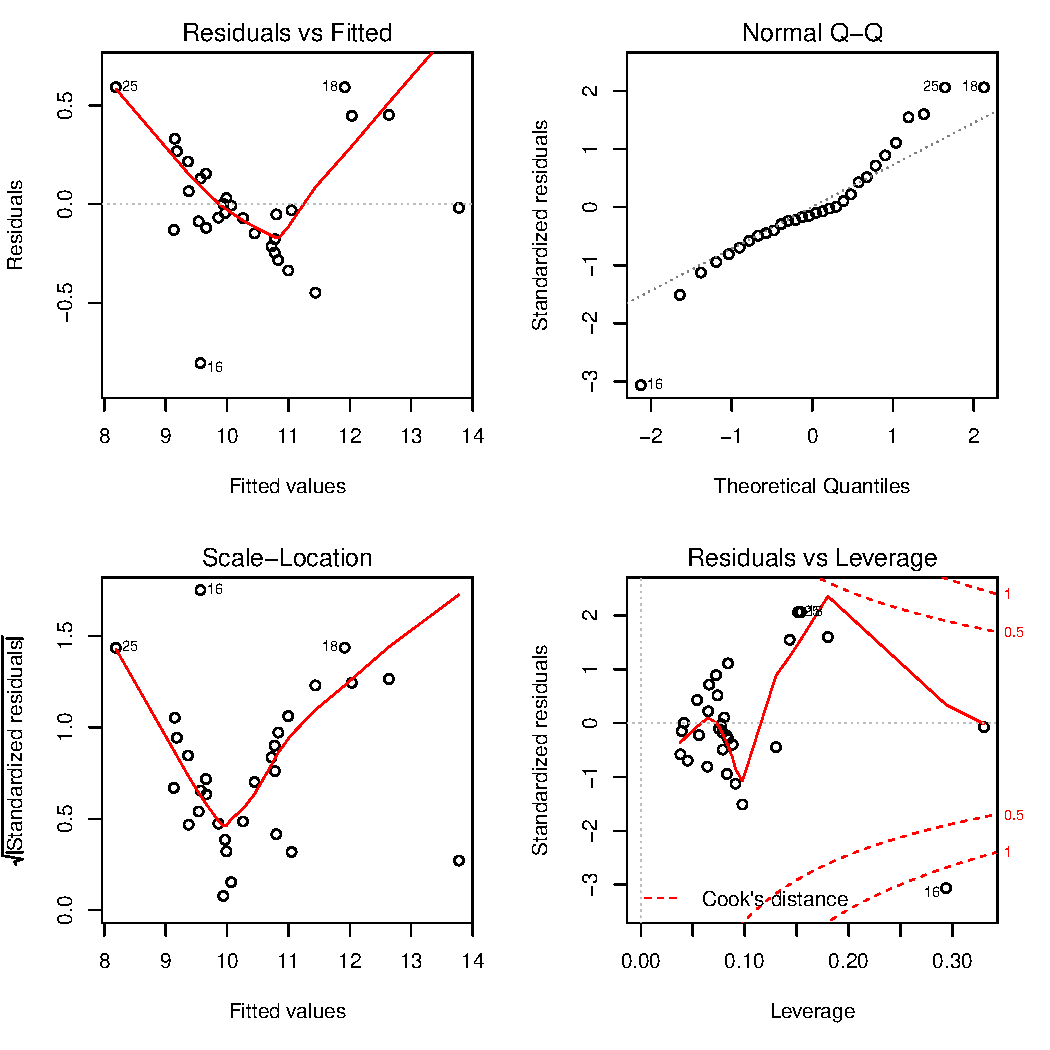
\includegraphics[width=0.6\linewidth]{figure/beamer-unnamed-chunk-27-1} 

}



\end{knitrout}
\end{frame}

%%%%%%%%%%%%%%%%%%%%%%%%%%%%%%%%%%%%%%%%%%%%%%%%%%%%%%%%%%%%%%%%%%%%%%%%%%%%%%%%%%%%%%%%%%%%%%%%%%%%


% %%%%%%%%%%%%%%%%%%%%%%%%%%%%%%%%%%%%%%%%%%%%%%%%%%%%%%%%%%%%%%%%%%%%%%%%%%%%%%%%%%%%%%%%%%%%%%%%%%%%
% \begin{frame}[fragile]{Conclusion}
% \begin{enumerate}
% \item R is a free and open source programming language for statistical computing and graphics.
% \item R contains many useful features for data analysis including data structures such as vectors and data frames that make it easy to perform statistical analysis and visualization.
% \item R is often used for hypothesis testing and understanding how to properly setup and interpret a test is an important skill.
% \end{enumerate}
% \end{frame}
% %%%%%%%%%%%%%%%%%%%%%%%%%%%%%%%%%%%%%%%%%%%%%%%%%%%%%%%%%%%%%%%%%%%%%%%%%%%%%%%%%%%%%%%%%%%%%%%%%%%%
% 

\begin{frame}{Conclusion}
\begin{itemize}
\item Like much of what we cover in this course, the materials reviewed here are to expose you the available tools for data analysis rather than provide all of the ``under the hood" details.
\item If you would like to learn more about the justifications behind using these statistical methods, I would suggest DATA 101 (more time and discussion on R and linear regression) STAT 230 (more discussions on statistical inference and hypothesis testing) and DATA 311 (machine learning). 
\end{itemize}
\end{frame}





\end{document}

